\section{Evaluation}
\label{sec:eval}

\begin{figure}[H]
    \centering
    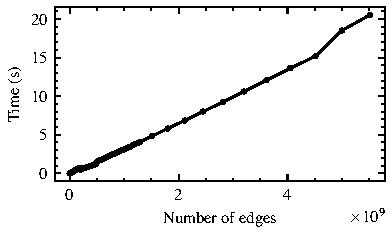
\includegraphics[width=\linewidth]{assets/timing.pdf}
    \caption{Timing}
    \label{fig:timing}
\end{figure}


% Based on the first 100,000 most frequently used words, we calculated the distance between every pair and visualized the graph using \href{https://gephi.org/}{Gephi's} ForceAtlas2 algorithm. The neighbors of the word \q{glace} and \q{prévoir} are shown in \autoref{fig:neighbors}. For bigger graphs than that, Gephi is not able to handle the amount of data anymore.

% Having translated the problem into a graph structure also allows us to use graph algorithms to discover interesting properties. As an example, Gephi implements the \textit{shortest path algorithm}: users can click on two words and the shortest path between them is calculated and shown in the graph. Beforehand, we filtered the graph to only include the most strong edges. With this, we can find chains like the following (read them aloud to hear the phonetic similarity):
% \begin{itemize}
%     \item trottoir $\rightarrow$ entrevoir $\rightarrow$ devoir $\rightarrow$ voire $\rightarrow$ voile $\rightarrow$ val $\rightarrow$ valait $\rightarrow$ fallait $\rightarrow$ falaise
%     \item falaise $\rightarrow$ fallait $\rightarrow$ palais $\rightarrow$ passais $\rightarrow$ dépassait $\rightarrow$ dépendait $\rightarrow$ répondait $\rightarrow$ répond $\rightarrow$ raison $\rightarrow$ maison
%     \item confusion $\rightarrow$ conclusion $\rightarrow$ exclusion $\rightarrow$ explosion $\rightarrow$ exposition $\rightarrow$ explications $\rightarrow$ respiration $\rightarrow$ précipitation $\rightarrow$ présentation $\rightarrow$ présenta $\rightarrow$ présente $\rightarrow$ présence $\rightarrow$ présidence $\rightarrow$ résidence $\rightarrow$ résistance $\rightarrow$ existence
% \end{itemize}

% todo lemma, lexeme
% https://en.wikipedia.org/wiki/Lemma_%28morphology%29
